\documentclass{article}
\usepackage{amssymb}
\usepackage{xcolor}
\usepackage{tcolorbox}
\usepackage{tikz}
\usetikzlibrary{decorations.pathreplacing}
\usetikzlibrary{calc}

\begin{document}

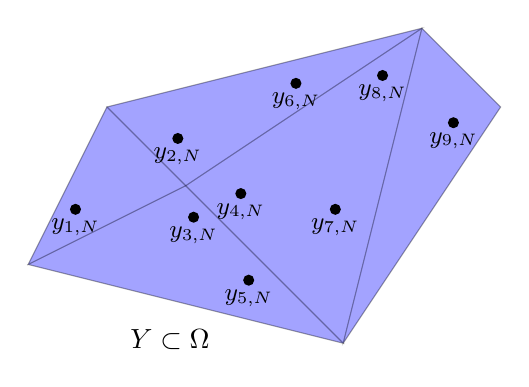
\begin{tikzpicture}

\filldraw[fill=blue, draw=black, opacity=0.2]
  (0,0) -- (4,-1) -- (6,2) -- (5,3)  -- (1,2)-- cycle;

\filldraw[fill=blue, draw=black, opacity=0.2]
  (0,0) -- (4,-1) -- (2,1) -- cycle;

\filldraw[fill=blue, draw=black, opacity=0.2]
 (4,-1)-- (5,3) -- (2,1) -- cycle;

\filldraw[fill=blue, draw=black, opacity=0.2]
 (5,3) -- (1,2) -- (2,1) -- cycle;

 \filldraw[fill=blue, draw=black, opacity=0.2]
 (1,2) -- (0,0) -- (2,1) -- cycle;

 \filldraw[fill=blue, draw=black, opacity=0.2]
 (5,3) -- (4,-1) -- (6,2) -- cycle;


 \fill (0.6,0.7) circle (2pt) node[below] {\small $y_{1,N}$};
 \fill (1.9,1.6) circle (2pt) node[below] {\small $y_{2,N}$};
 \fill (2.1,0.6) circle (2pt) node[below] {\small $y_{3,N}$};
 \fill (2.7,0.9) circle (2pt) node[below] {\small $y_{4,N}$};
 \fill (2.8,-0.2) circle (2pt) node[below] {\small $y_{5,N}$};
  \fill (3.4,2.3) circle (2pt) node[below] {\small $y_{6,N}$};
 \fill (3.9,0.7) circle (2pt) node[below] {\small $y_{7,N}$};
  \fill (4.5,2.4) circle (2pt) node[below] {\small $y_{8,N}$};
  \fill (5.4,1.8) circle (2pt) node[below] {\small $y_{9,N}$};


  \node[below] at (1.8,-0.7)  {$Y \subset \Omega$};

\end{tikzpicture}

\end{document}